\documentclass[a4paper,oneside,11pt,article]{memoir}

% This preamble is written by Amalie Stokholm with the help and inspiration from Steffen Videbæk, Mathias Rav, Rasmus Villemoes and Lars 'daleif' Madsen. 

% Check input
\usepackage[utf8]{inputenc}
\usepackage[T1]{fontenc}

% Fonts and microtype
\usepackage[danish,english]{babel}
\usepackage{lmodern}
\usepackage[final]{microtype}

\usepackage{url}
\usepackage{xspace}

% Graphics
\usepackage{graphicx}

% Mathematics
\usepackage{amsmath}

% References
\usepackage{varioref}
\usepackage[colorlinks=true,
			allcolors=black
			]{hyperref}
\usepackage{cleveref}

% Syntaxmarking: c
% Defining colors
\usepackage{color}
	\definecolor{deepblue}{rgb}{0,0,0.5}
	\definecolor{deepred}{rgb}{0.6,0,0}
	\definecolor{deepgreen}{rgb}{0,0.5,0}
\usepackage{listings}
% PDF accessibility support for literate listings
\usepackage{accsupp}
	\lstset{
			language=c,
			basicstyle=\small\sffamily,
			keywordstyle=\color{deepblue},  
			emphstyle=\color{deepred},    
			stringstyle=\color{deepgreen},
			commentstyle=\color{red},        
			showstringspaces=false,
			columns=fullflexible,
			keepspaces=true,
			numbers=left,
			numbersep=20pt,
			numberstyle=\tiny,
			% escapeinside={$}{$},
			% mathescape=true,
			literate=
			{_}{%
			  \makebox[0pt][l]{%
			    \makebox[4pt][c]{%
			      \textcolor{white}{\_}}}%
			  \rule[-0.4pt]{4pt}{0.4pt}%
			}1
			{-}{%
			  % http://tex.stackexchange.com/a/18509/76220
			  % Use accessibility support to change what text
			  % is copied out of the PDF: ASCII hyphen
			  % instead of Unicode minus
			  \BeginAccSupp{
			    method=escape,
			    ActualText={-}
			  }%
			  $-$%
			  \EndAccSupp{}%
			}1
			{*}{%
			  % http://tex.stackexchange.com/a/18509/76220
			  % Use accessibility support to change what text
			  % is copied out of the PDF: ASCII hyphen
			  % instead of Unicode minus
			  \BeginAccSupp{
			    method=escape,
			    ActualText={*}
			  }%
			  $*$%
			  \EndAccSupp{}%
			}1
			{µ}{$\mu$}1
			{É}{{\'E}}1,
}

% Margins (with help from Steffen Videbæk)
\setlxvchars
\setulmargins{*}{*}{1.618}
\setlrmargins{*}{*}{1}
\checkandfixthelayout[nearest] % needed in order for memoir to compile these settings correctly.

\begin{document}
\begin{center}
  \sffamily
    {\Large Exam in Practical Programming} \\
    \vspace{.8em}
    {Amalie Louise Stokholm, 201303663, \texttt{stokholm@phys.au.dk}} \\
  {\today}
\end{center}
\subsection*{Will these functions leak memory?}
\begin{lstlisting}
void stat() {
	double a[500];
}
\end{lstlisting}
The functions as \url{stat} stores the temporary variables in the stack. The stack has size limits, but a size of $500$ is probably not big enough to hit this limit. The stack grows and shrinks in memory as the function pushes more variables to it, but the stack is user-friendly as the variables are allocated and freed automatically. As soon as the function has finished, the variables are freed from the stack, the memory is re-usable, and thus there is no memory leak.
\begin{lstlisting}
void vla(size_t n) {
	double a[n];
}
\end{lstlisting}
This function \url{vla} uses as \url{stat} the stack to store memory. When the function is done, the variables are freed from the stack and the memory can be reused. Just as \url{stat}, this function does not leak memory.
\begin{lstlisting}
void mal() {
	double* a = (double*) malloc(500 * sizeof(double));
}
\end{lstlisting}
In contrast to \url{stat} and \url{vla}, the next couple of functions use the heap, where memory is not managed automatically for the user. The user needs to manually allocate and free memory in order to avoid memory leak. In \url{mal}, the memory is only allocated, but not freed, and therefore there is a memory leak as this leads to a build-up of non-reusable memory.
\begin{lstlisting}
void maf() {
	double* a = (double*) malloc(500 * sizeof(double));
	free(a);
}
\end{lstlisting}
This function \url{maf} uses the heap, but in contrast to \url{mal}, the memory is both allocated and freed. A memory leak is thus avoided as all the memory can be reused.
\begin{lstlisting}
double* mar() {
	double* a = (double*) malloc(500 * sizeof(double));
	return a;
}
\end{lstlisting}
In \url{mar}, there is no memory leak as it returns a pointer. A function calling this function can reuse the memory allocated by $a$ by using this pointer.

\clearpage
\subsection*{Problem}
Implement the Bessel function of the first kind of integer index using Bessel’s integral
representation.
\begin{equation}
J_n(x) = \frac{1}{\pi} \int_{0}^{\pi} \cos(nt - x \sin(t))\,\text{d}t.
\label{eq:bessel}
\end{equation}
Compare with the corresponding function from \url{<math.h>} or from GSL.
\plainbreak1
In the \url{Makefile}, can four parameters be defined: the index $n$, $x_{\text{start}}$, $x_{\text{end}}$, and $x_{\text{delta}}$. This allows the user to determine the index of the Bessel function of the first kind and the range of $x$-values wanted for the computation. The \url{Makefile} takes care of generating the properties of the plot (Fig.\@~\ref{fig:plot}), the clean-up routine, and the compilation and linking of the \url{jn.c} into the executable file \url{./jn}.

\url{jn.c} contains Eq.\@~\ref{eq:bessel} in the appropriate form for \url{gsl_integration_qag}, which is the used integration procedure. In two for loops, the value from the integration method and the value from \url{<math.h>} is printed and thus saved in out.txt. In order to check whether the two values are equal, a check is implemented and the result from this test is piped into stderr.

\begin{figure} [b!]
\centering
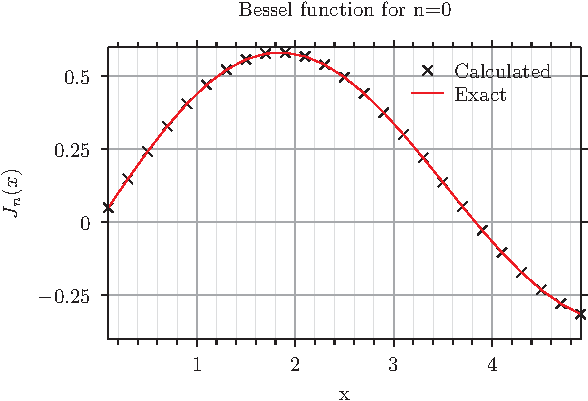
\includegraphics[width=1\linewidth]{plot}
\caption{Comparison between the calculated $J_n(x)$ (points) and $J_n(x)$ from \url{<math.h>} (lines) for a given $n$.}
\label{fig:plot}
\end{figure}

\end{document}